\appendix
\chapter{Artefactos software}

Este apéndice recoge los principales artefactos software generados durante el desarrollo del Trabajo de Fin de Grado. Su inclusión complementa la memoria principal con una vista técnica de los entregables reales del proyecto.

Además, se proporciona un enlace al repositorio de GitHub donde se encuentra el código fuente completo del videojuego: https://github.com/nsh255/ascension.git

\section{Estructura del proyecto}

El proyecto se ha desarrollado en Unity con una organización modular orientada a responsabilidades. A nivel práctico, los artefactos más relevantes del repositorio son:

\begin{itemize}
    \item \textbf{Ascension/Ascension/Assets/Scripts}: lógica principal del juego en C\#, organizada por subsistemas (Core, Player, Enemies, Weapons, UI, Tiles y LevelGeneration).
    \item \textbf{Ascension/Ascension/Assets/Prefabs}: objetos reutilizables del juego (jugador, enemigos, armas, escaleras y elementos de sala).
    \item \textbf{Ascension/Ascension/Assets/Scenes}: escenas del flujo completo (menú principal, selección de class y escena principal de juego).
    \item \textbf{Ascension/Ascension/LATEX/Diagramas}: fuentes PlantUML de los diagramas técnicos utilizados en la memoria.
    \item \textbf{Ascension/Ascension/LATEX}: memoria final, bibliografía y figuras integradas para compilación del documento.
\end{itemize}

Esta estructura ha permitido mantener bajo acoplamiento entre módulos y facilitar la iteración de mecánicas.

\section{Arquitectura del sistema}

La arquitectura del videojuego se basa en un enfoque modular con patrones \textit{Singleton}, \textit{Observer}, \textit{Strategy} y \textit{Template Method}. Entre los subsistemas implementados destacan:

\begin{itemize}
    \item Gestión de estado global de partida (\texttt{GameManager}).
    \item Progresión de salas y coordinación de oleadas (\texttt{RoomFlowController} y \texttt{EnemyManager}).
    \item Generación procedural de salas y tiles con efectos (\texttt{RoomGenerator} y \texttt{FloorTileManager}).
    \item Sistema de jugador, combate y armas (cuerpo a cuerpo y a distancia).
    \item Interfaz de usuario y persistencia de puntuaciones.
\end{itemize}

Con el objetivo de aportar una visión estructural del sistema, en el siguiente apartado se incluyen los diagramas UML utilizados durante el diseño.

\section{Diagramas del sistema}

La Figura \ref{fig:clases} muestra el diagrama de clases del sistema, en el que se representan las principales entidades del videojuego y sus relaciones. Este diagrama permite comprender la organización interna del código y la separación de responsabilidades entre los distintos componentes.

\clearpage
\begin{sidewaysfigure}
    \begin{center}
    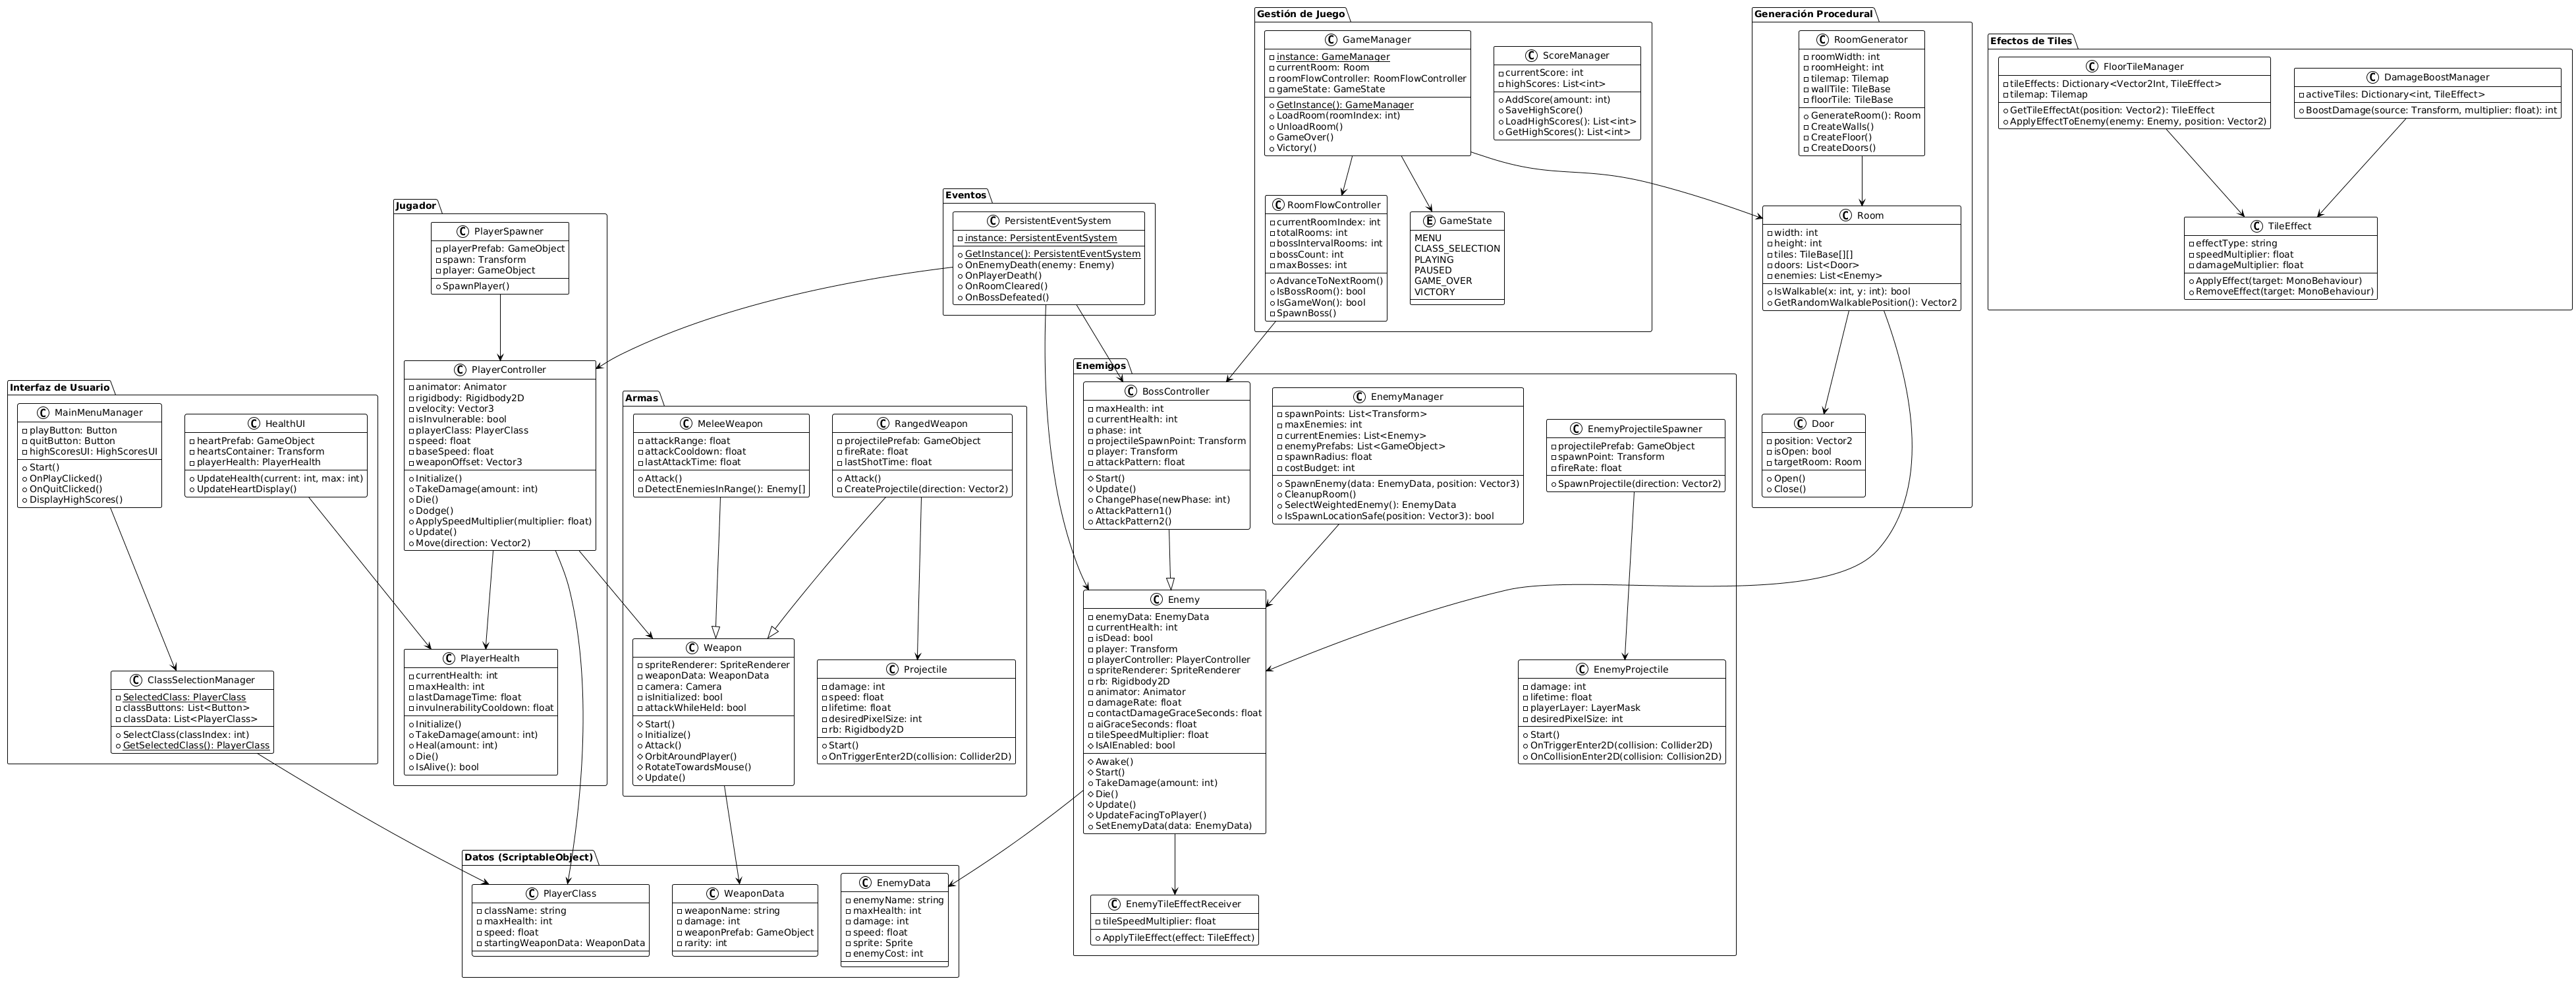
\includegraphics[width=\textheight]{Figuras/Diagrama_Clases.png}
    \caption{Diagrama de clases del sistema}
    \label{fig:clases}
    \end{center}
\end{sidewaysfigure}
\clearpage

Por otro lado, la Figura \ref{fig:casosuso} presenta el diagrama de casos de uso, que describe las interacciones principales entre el jugador y el sistema, proporcionando una visión funcional del comportamiento esperado del videojuego.

\clearpage
\begin{sidewaysfigure}
    \begin{center}
    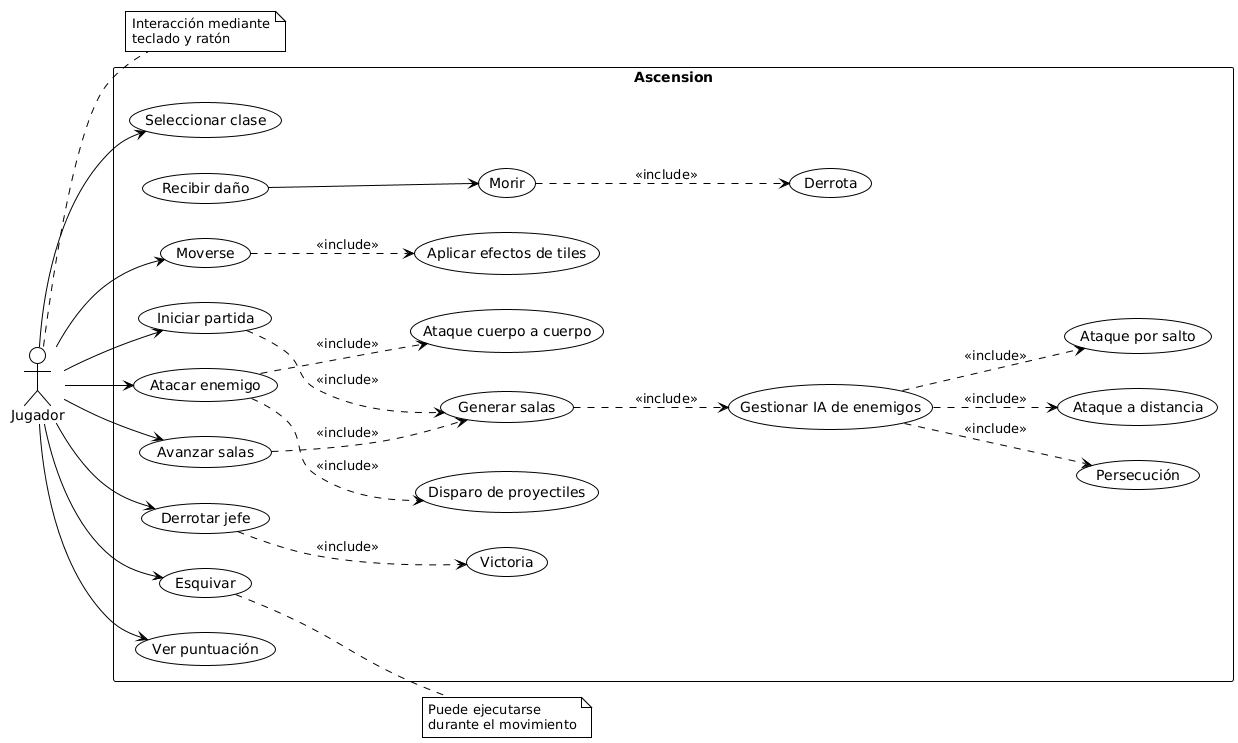
\includegraphics[width=\textheight]{Figuras/Diagrama_Casos_Uso.png}
    \caption{Diagrama de casos de uso del sistema}
    \label{fig:casosuso}
    \end{center}
\end{sidewaysfigure}
\clearpage

